% --------------------------------------------------------------------
% Document structure
% --------------------------------------------------------------------
\documentclass[paper=a4, fontsize=12pt]{report}


% --------------------------------------------------------------------
% Packages
% --------------------------------------------------------------------
\usepackage[a4paper]{geometry}
%\usepackage[margin=1in, left=1.5in]{geometry}
\usepackage[hidelinks]{hyperref}
\usepackage[utf8]{inputenc}
\usepackage[T1]{fontenc}
\usepackage{lipsum}
\usepackage{lastpage}
\usepackage{fancyhdr}
\usepackage{caption}
\usepackage{subcaption}

% Title packages
\usepackage{titlesec}
\titleformat{\chapter}{\normalfont\huge\bfseries}{\thechapter. }{0pt}{\Huge}
\titlespacing{\chapter} {0pt}{0pt}{10pt}

% Table packages
\usepackage[none]{hyphenat}
\usepackage{tabularx}
\usepackage{multirow}
\captionsetup[table]{skip=5pt}

% Graphics packages
\usepackage{graphicx}
\usepackage{float}
\graphicspath{images/}








% --------------------------------------------------------------------
% Variables
% --------------------------------------------------------------------
% Title page variables
\def \SubTitleVar {A LaTeX report starting point}
\def \DateVar {\today}
\def \TitleVar {\LaTeX-quickstart}
\def \AuthorVar {Rick van Lieshout}
\def \AuthorTitleVar {Software Engineer}
\def \AuthorURLVar {http://mastermindzh.com}
\def \AuthorEmailVar {info@rickvanlieshout.com}

% General variables


% --------------------------------------------------------------------
% Includes
% --------------------------------------------------------------------
\newcommand{\HRule}[1]{\rule{\linewidth}{#1}} 	% Horizontal rule
\newcommand{\printTitlePage}{
	\thispagestyle{empty}		% Remove page numbering on this page
	\printtitle					% Print the title data as defined above
	\vfill						% Variable fill
	\printauthor				% Print the author data as defined above
	\newpage
}

\makeatletter								% Title
\def\printtitle{%						
	{\centering \@title\par}}
\makeatother									

\makeatletter								% Author
\def\printauthor{%					
	{\flushright \large \@author}}				
\makeatother							

\title{	\normalsize \textsc{\SubTitleVar} 	% Subtitle
	\\[2.0cm]								% 2cm spacing
	\HRule{0.5pt} \\						% Top line
	\LARGE \textbf{\uppercase{\TitleVar}}	% Title
	\HRule{2pt} \\ [0.5cm]					% Lower line + 0.5cm spacing
	\normalsize \DateVar					% Todays date
}

\author{
	\AuthorVar\\	
	\AuthorTitleVar\\	
	\url{\AuthorURLVar}\\
	\href{mailto:\AuthorEmailVar}{\AuthorEmailVar}\\
}


\begin{document}
	\begin{titlepage}
		\printTitlePage		
	\end{titlepage}
	% --------------------------
	% Front matter (includes introduction)
	% --------------------------
	\pagenumbering{roman}

\chapter*{Abstract}\label{sec:abstract}
% generate random text to fill the page :)
\lipsum[1]
\addcontentsline{toc}{chapter}{\numberline{}Abstract}

\chapter*{Acknowledgements}\label{sec:acks}
% generate random text to fill the page :)
\lipsum[1]
\addcontentsline{toc}{chapter}{\numberline{}Acknowledgements}

% Table of Contents
\tableofcontents
\listoffigures \label{list:listOfFigures}
\addcontentsline{toc}{chapter}{\numberline{}List of figures}
\listoftables \label{list:listOfTables}
\addcontentsline{toc}{chapter}{\numberline{}List of tables}


\chapter{Introduction}\label{sec:introduction}
% generate random text to fill the page :)
\lipsum[1]
\setcounter{page}{1}
	\fancypagestyle{plain}{
	\fancyfoot[R]{Page \thepage\ of \pageref{LastPage}}
}
\cfoot{}
\pagenumbering{arabic}
\pagestyle{plain}

	% --------------------------
	% Main matter
	% --------------------------
	\chapter{Text test chapter}\label{sec:first}
	% generate random text to fill the page :)
\lipsum[1]

\section{First section with a very \\long name for testing purposes}
The introduction can be found on page \pageref{sec:introduction}.
\subsection{First subsection}
\lipsum[1-3]

\subsection{Second subsection (with footnotes)}
This\footnote{\url{google.com}} line of text will have multiple\footnote{\url{google.com}} footnotes all pointing to google.com\footnote{\url{google.com}}.

\subsubsection{first subsubsection}
\lipsum[1]
\cite{first}

	
	\chapter{Elements test chapter}\label{sec:second}
	% generate random text to fill the page :)
\lipsum[1]

\section{Images}
Behold this beautiful floating figure:

\begin{figure}[H]
	% always put label neat the top (after caption!) or your reference will not work as expected.
	\caption[Programming is magic]{Programming is magic} 
	\label{fig:programmingMagic} 
	\centering
	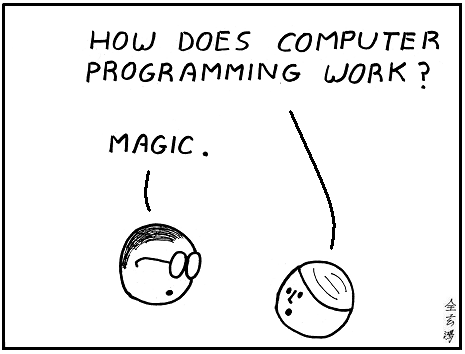
\includegraphics[height=300px]{images/programming.png}
	% caption[Optional caption][Local caption] References ONLY go in the local caption!

\end{figure}

\subsection{Solid evidence}
Figure \ref{fig:programmingMagic} proves that programming is magic.

\subsection{Multiple images}
\begin{figure}[H]
	\centering
	\begin{subfigure}[b]{0.3\textwidth}
		\centering
		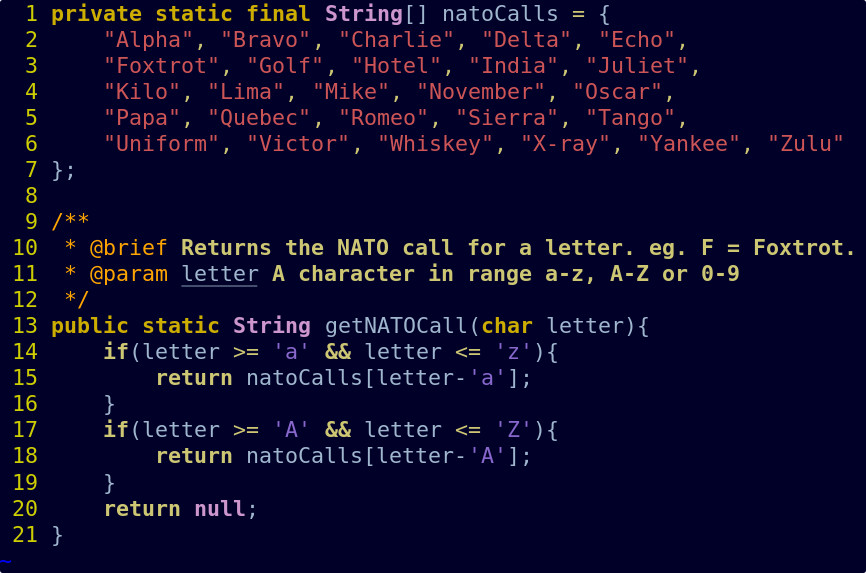
\includegraphics[width=\textwidth]{images/programmingLanguages/java.jpg}
		\caption{Java}
		\label{Java}
	\end{subfigure}
	\hfill
	\begin{subfigure}[b]{0.3\textwidth}
		\centering
		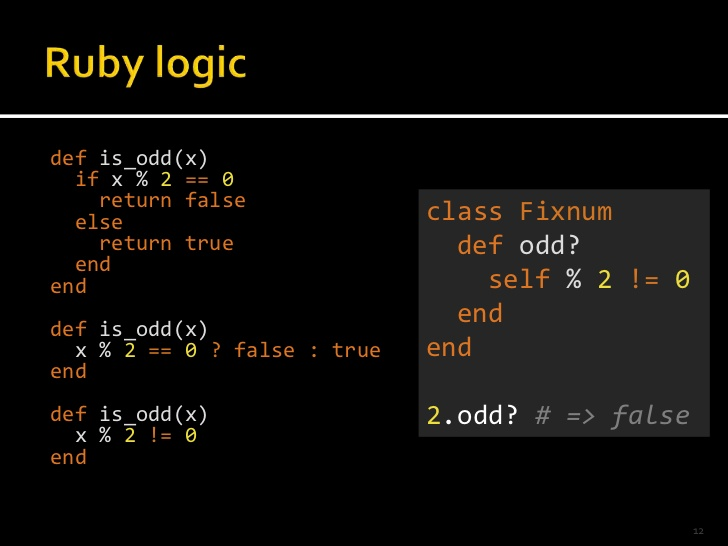
\includegraphics[width=\textwidth]{images/programmingLanguages/ruby.jpg}
		\caption{Ruby}
		\label{fig:ruby}
	\end{subfigure}
	\hfill
	\begin{subfigure}[b]{0.3\textwidth}
		\centering
		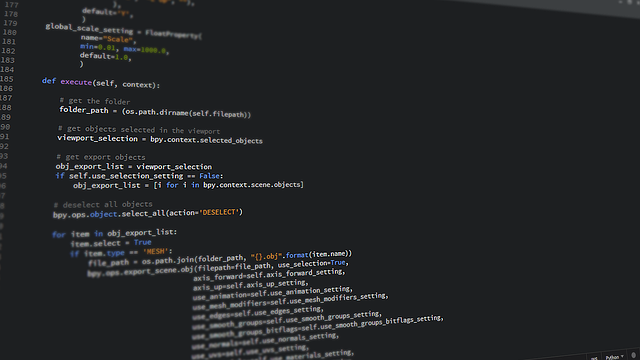
\includegraphics[width=\textwidth]{images/programmingLanguages/python.png}
		\caption{Python}
		\label{fig:python}
	\end{subfigure}
	\caption{Three programming languages}
	\label{fig:three graphs}
\end{figure}


\section{Tables}
Down below you'll find a couple of tables.
\begin{table}[H]
	\label{tab:basicTable}
	\centering
	\caption[A basic table]{A basic table}
	\begin{tabular}{l c r} %alignments
		Language & Compiled & Difficulty \\ \hline	
		Javascript & \ & easy \\
		Ruby / Python & \ & normal \\
		Java & X & hard \\
		Scala & X & nightmare \\
	\end{tabular}
\end{table}


\subsection{A series of tables}


\begin{table}[H]
	\label{tab:knotsAndCrosses}
	\centering
	\caption[Three Knots and Crosses games]{Three Knots and Crosses games}
	\begin{tabular}{|c | c | c|} %alignments
		\hline
		O & X & O \\\hline
		X & O & X \\\hline
		X & O & X \\\hline 
	\end{tabular}
	\begin{tabular}{|c | c | c|} %alignments
		\hline
		O & X & - \\\hline 	
		X & O & - \\\hline
		- & - & O \\\hline 
	\end{tabular}
	\begin{tabular}{|c | c | c|} %alignments
		\hline
		X & O & X \\\hline 	
		O & X & O \\\hline
		O & X & O \\\hline 
	\end{tabular}
\end{table}


\subsection{Complicated tables}
\begin{table}[H]
	\label{tab:complicatedTable}
	\centering
	\def\arraystretch{1.5} % padding
	\caption[A complicated table]{A complicated table generated with: \url{http://www.tablesgenerator.com}}
\begin{tabular}{|l|c|c|c|c|}
	\hline
	\textbf{Language} & \multicolumn{1}{l|}{\textbf{typing}} & \multicolumn{1}{l|}{\textbf{Object oriented}} & \multicolumn{1}{l|}{\textbf{GC}} & \multicolumn{1}{l|}{\textbf{Difficulty}} \\ \hline
	Javascript & dynamic &  & X & easy \\ \hline
	Ruby/Python & dynamic & X & X & normal \\ \hline
	\multicolumn{5}{|c|}{\textit{\textbf{Compiled languages}}} \\ \hline
	Java & static & X & X & hard \\ \hline
	Scala & dynamic & X & X & nightmare \\ \hline
\end{tabular}
\end{table}
\begin{table}[H]
	\label{tab:unitConversion}
	\centering
	\caption[Unit conversion table]{Unit conversion table}
	\begin{tabular}{|r|l|}
		\hline
		7C8 & hexadecimal \\
		3710 & octal \\ \cline{2-2}
		11111001000 & binary \\
		\hline \hline
		1992 & decimal \\
		\hline
	\end{tabular}
\end{table}

\begin{table}[H]
	\label{tab:unitConversion}
	\centering
	\caption[Spanning in both directions simultaneously]{Spanning in both directions simultaneously}
	\begin{tabular}{cc|c|c|c|c|l}
		\cline{3-6}
		& & \multicolumn{4}{ c| }{Primes} \\ \cline{3-6}
		& & 2 & 3 & 5 & 7 \\ \cline{1-6}
		\multicolumn{1}{ |c  }{\multirow{2}{*}{Powers} } &
		\multicolumn{1}{ |c| }{504} & 3 & 2 & 0 & 1 &     \\ \cline{2-6}
		\multicolumn{1}{ |c  }{}                        &
		\multicolumn{1}{ |c| }{540} & 2 & 3 & 1 & 0 &     \\ \cline{1-6}
		\multicolumn{1}{ |c  }{\multirow{2}{*}{Powers} } &
		\multicolumn{1}{ |c| }{gcd} & 2 & 2 & 0 & 0 & min \\ \cline{2-6}
		\multicolumn{1}{ |c  }{}                        &
		\multicolumn{1}{ |c| }{lcm} & 3 & 3 & 1 & 1 & max \\ \cline{1-6}
	\end{tabular}
\end{table}

	
	% --------------------------
	% Back(end) matter
	% --------------------------
	
\end{document}